% -*- latex -*-

\chapter{Introduction}
\label{chap:Introduction}

High-performance computing relies on ever finer threading. Advances in
processor technology include ever greater numbers of cores, hyperthreading,
accelerators with integrated blocks of cores, and special vectorized
instructions, all of which require more software parallelism to achieve
peak performance. Traditional visualization solutions cannot support this
extreme level of concurrency. Extreme scale systems require a new
programming model and a fundamental change in how we design algorithms. To
address these issues we created VTK-m: the visualization toolkit for
multi-/many-core architectures.

VTK-m supports a number of algorithms and the ability to design further
algorithms through a top-down design with an emphasis on extreme
parallelism. VTK-m also provides support for finding and building links
across topologies, making it possible to perform operations that determine
manifold surfaces, interpolate generated values, and find adjacencies.
Although VTK-m provides a simplified high-level interface for programming,
its template-based code removes the overhead of abstraction.

\begin{figure}[htb]
  \centering
  %% \begin{tabular}{ccc}
  %%   CUDA SDK & PISTON & VTK-m \\
  %%   {\small 431 LOC} & {\small 369 LOC} & {\small 265 LOC} \\
  %%   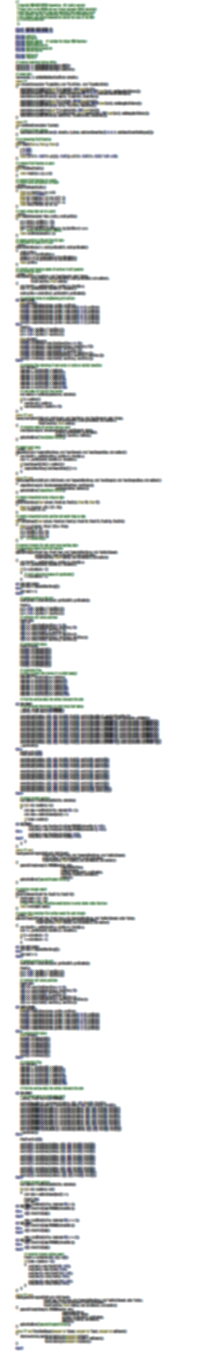
\includegraphics[width=.75in]{images/MCCompareCuda} &
  %%   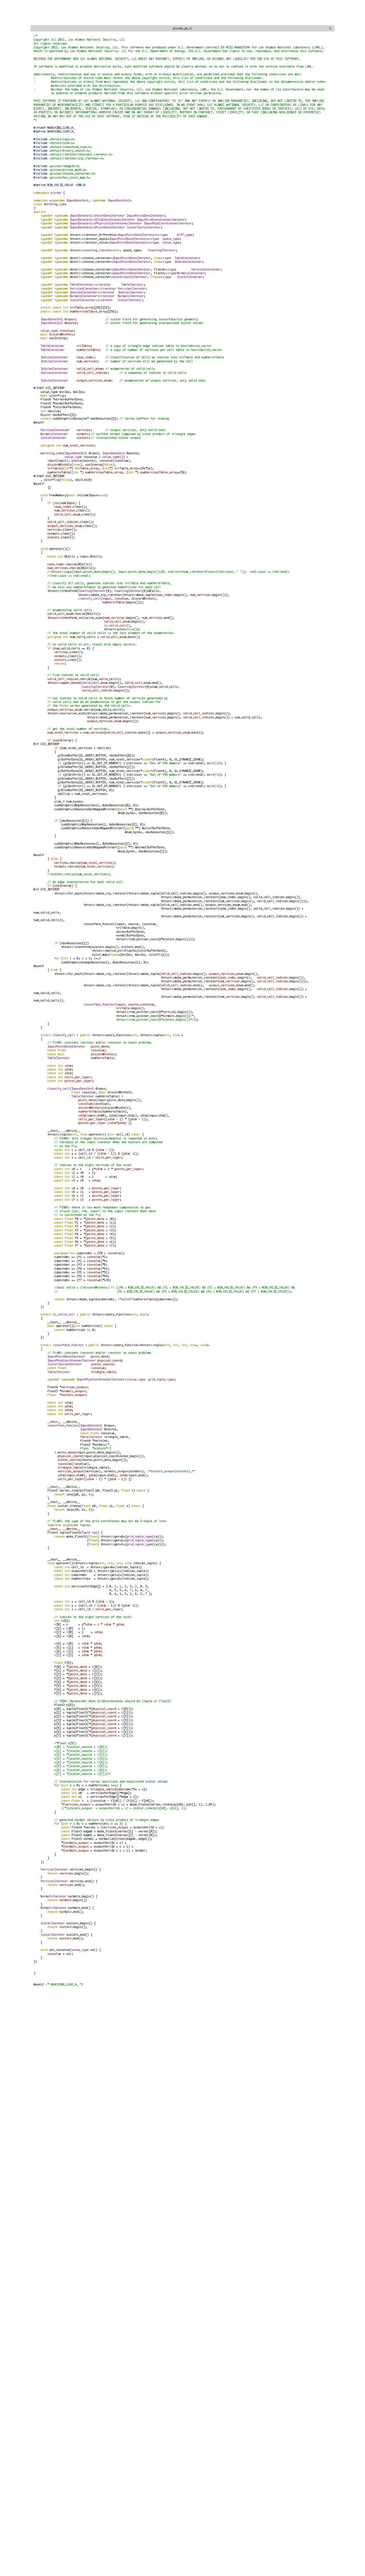
\includegraphics[width=.75in]{images/MCComparePiston} &
  %%   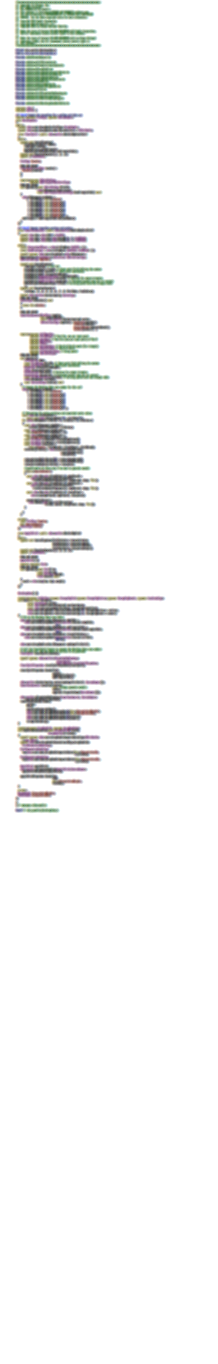
\includegraphics[width=.75in]{images/MCCompareVTKm}
  %% \end{tabular}
  \begin{tabular}{cc}
    CUDA SDK & VTK-m \\
    {\small 431 LOC} & {\small 265 LOC} \\
    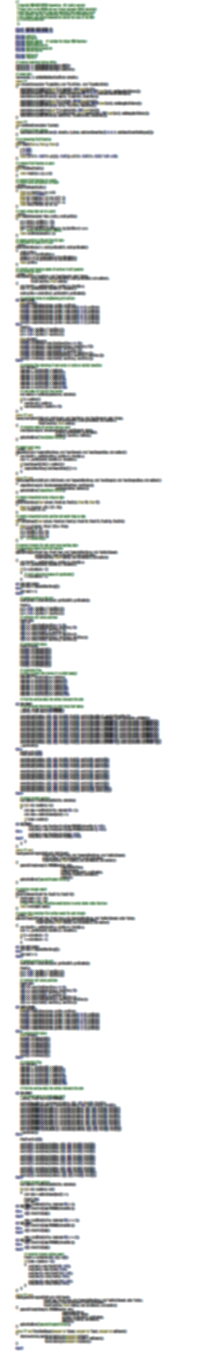
\includegraphics[width=.75in]{images/MCCompareCuda} &
    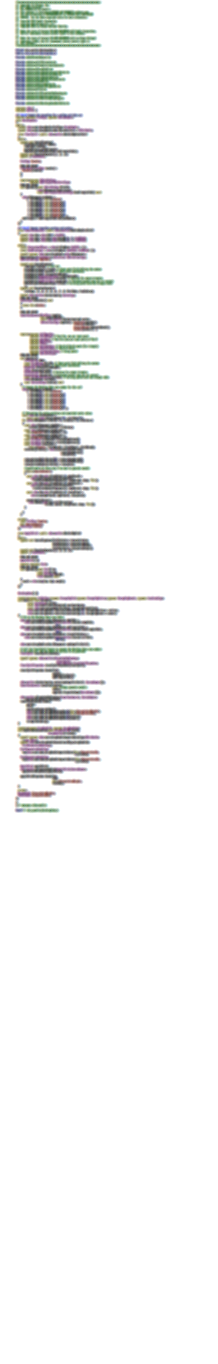
\includegraphics[width=.75in]{images/MCCompareVTKm}
  \end{tabular}
  \caption[Comparison of Marching Cubes implementations.]{
    Comparison of the Marching Cubes algorithm in VTK-m and the reference implementation in the CUDA SDK.
    Implementations in VTK-m are simpler, shorter, more general, and easier to maintain.
    (Lines of code (LOC) measurements come from cloc.)}
  \label{fig:MCCompare}
\end{figure}

VTK-m simplifies the development of parallel scientific visualization algorithms by providing a framework of supporting functionality that allows developers to focus on visualization operations.
Consider the listings in Figure~\ref{fig:MCCompare} that compares the size of the implementation for the Marching Cubes algorithm in VTK-m with the equivalent reference implementation in the CUDA software development kit.
Because VTK-m internally manages the parallel distribution of work and data, the VTK-m implementation is shorter and easier to maintain.
Additionally, VTK-m provides data abstractions not provided by other libraries that make code written in VTK-m more versatile.

\begin{didyouknow}
  VTK-m is written in C++ and makes extensive use of templates. The toolkit
  is implemented as a header library, meaning that all the code is
  implemented in header files (with extension \textfilename{.h}) and
  completely included in any code that uses it. This allows the compiler to
  inline and specialize code for better performance.
\end{didyouknow}

\section{How to Use This Guide}

This user's guide is organized into three parts to help guide novice to
advanced users and to provide a convenient reference.
Part~\ref{part:GettingStarted}, Getting Started, provides everything needed
to get up and running with VTK-m. In this part we learn the basics of
reading and writing data files, using filters to process data, and perform
basic rendering to view the results.

Part~\ref{part:Using}, Using VTK-m, dives deeper into the VTK-m library and
provides all the information needed to customize VTK-m's data structures
and support multiple devices.

Part~\ref{part:Developing}, Developing with VTK-m, documents how to use
VTK-m's framework to develop new or custom visualization algorithms. This
part describes how worklets are used to implement and execute algorithms
and how to use worklets to implement new filters.
Part~\ref{part:Developing} also describes the facilities available in the
execution environment that help write visualization algorithms.

Part~\ref{part:Advanced}, Advanced Development, exposes the inner workings
of VTK-m and allows you to design new algorithmic structures not already
available. \fix{This might be removed in the first version of the book.}

\section{Conventions Used in This Guide}

When documenting the VTK-m API, the following conventions are used.
\begin{itemize}
\item Filenames are printed in a \textfilename{sans serif font}.
\item C++ code is printed in a \textcode{monospace font}.
\item Macros and namespaces from VTK-m are printed in \textnamespace{red}.
\item Identifiers from VTK-m are printed in \textidentifier{blue}.
\item Signatures, described in Chapter~\ref{chap:Worklets}, and the
  tags used in them are printed in \textsignature{green}.
\end{itemize}

This guide provides actual code samples throughout its discussions to
demonstrate their use. These examples are all valid code that can be
compiled and used although it is often the case that code snippets are
provided. In such cases, the code must be placed in a larger context.

\begin{didyouknow}
  In this guide we periodically use these \textbf{Did you know?} boxes to
  provide additional information related to the topic at hand.
\end{didyouknow}

\begin{commonerrors}
  \textbf{Common Errors} blocks are used to highlight some of the common
  problems or complications you might encounter when dealing with the topic
  of discussion.
\end{commonerrors}
